\documentclass[12pt]{article}
	
\title{CSC 320 - Worksheet 6}
\author{Nadeem Abdul Hamid}
\date{March 26, 2024}  


\usepackage[margin=1in]{geometry}		% For setting margins
\usepackage{amsmath}				% For Math
\usepackage{amsthm}
\usepackage{fancyhdr}				% For fancy header/footer
\usepackage{graphicx}				% For including figure/image
\usepackage{cancel}					% To use the slash to cancel out stuff in work
\usepackage[shortlabels]{enumitem}
\usepackage{hyperref}
\usepackage{jigsaw}

\usepackage{algorithm,caption}
\usepackage{algpseudocodex}
% docs: https://ctan.math.washington.edu/tex-archive/macros/latex/contrib/algpseudocodex/algpseudocodex.pdf


%%%%%%%%%%%%%%%%%%%%%%
% Set up fancy header/footer
% taken from https://www.overleaf.com/latex/templates/homework-template/yvgnmrbywwnp
\makeatletter    % for \@ in \@title
\pagestyle{fancy}
\fancyhead[LO,L]{\@author}
\fancyhead[CO,C]{\@title}
\fancyhead[RO,R]{\@date}
\fancyfoot[LO,L]{}
\fancyfoot[CO,C]{\thepage}
\fancyfoot[RO,R]{}
\renewcommand{\headrulewidth}{0.4pt}
\renewcommand{\footrulewidth}{0.4pt}
\makeatother    % restore
%%%%%%%%%%%%%%%%%%%%%%


%%%%%%%%%%%%%%%%%%%%%%
% from: https://tex.stackexchange.com/questions/14667/does-latex-define-a-semantic-equivalent-of-textbf
\makeatletter
\newcommand{\strong}[1]{\@strong{#1}}
\newcommand{\@@strong}[1]{\textbf{\let\@strong\@@@strong#1}}
\newcommand{\@@@strong}[1]{\textnormal{\let\@strong\@@strong#1}}
\let\@strong\@@strong
\makeatother
%%%%%%%%%%%%%%%%%%%%%%


\newcommand{\emptybox}[2][\textwidth]{%
  \begingroup
  \setlength{\fboxsep}{-\fboxrule}%
  \noindent\framebox[#1]{\rule{0pt}{#2}}%
  \endgroup
}

\newtheorem{theorem}{Theorem}
\newtheorem{lemma}{Lemma}


\begin{document}

\section{Graphs}
\subsection{Whatever-first search}

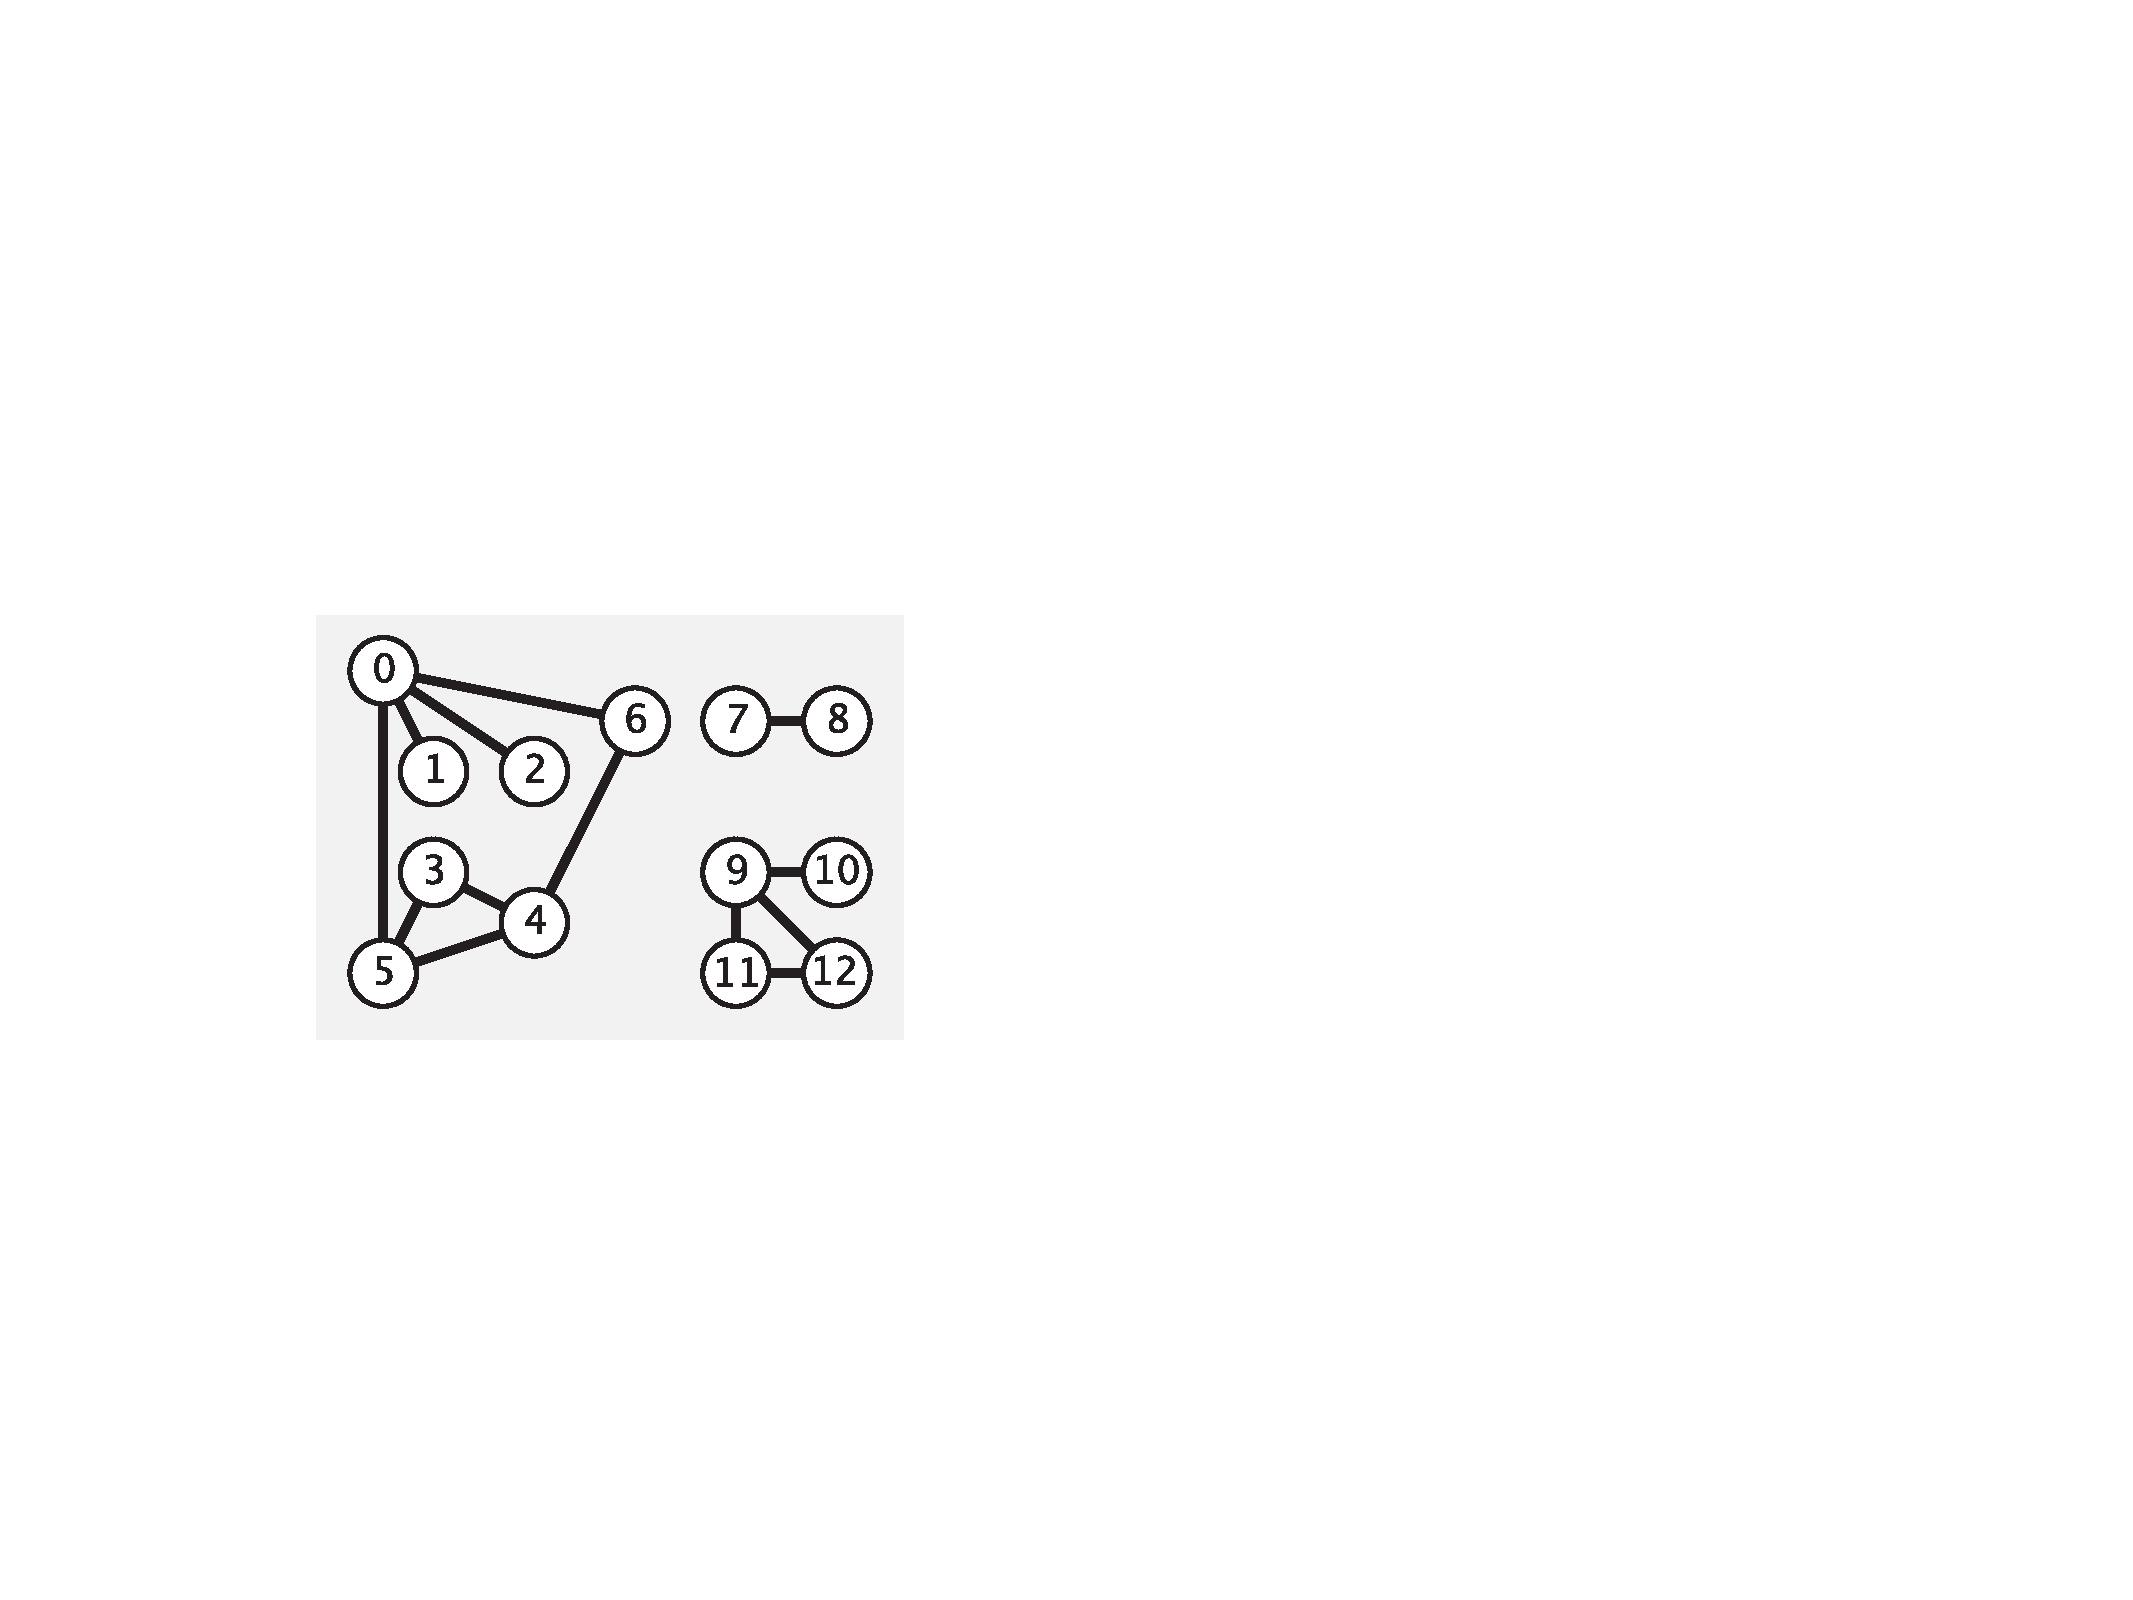
\includegraphics{w07-graph1.pdf}

Perform \textsc{WhateverFirstSearch} (page 200) on the graph above, starting with $S=0$ and processing nodes in numerical order in case of deciding what to take next, with the following "bag" variants:

\begin{itemize}
    \item Stack (what specialized search is this?)
    \item Queue (what specialized search is this?)
    \item Priority Queue, on this edge-weighted graph:
    
    \begin{center}
        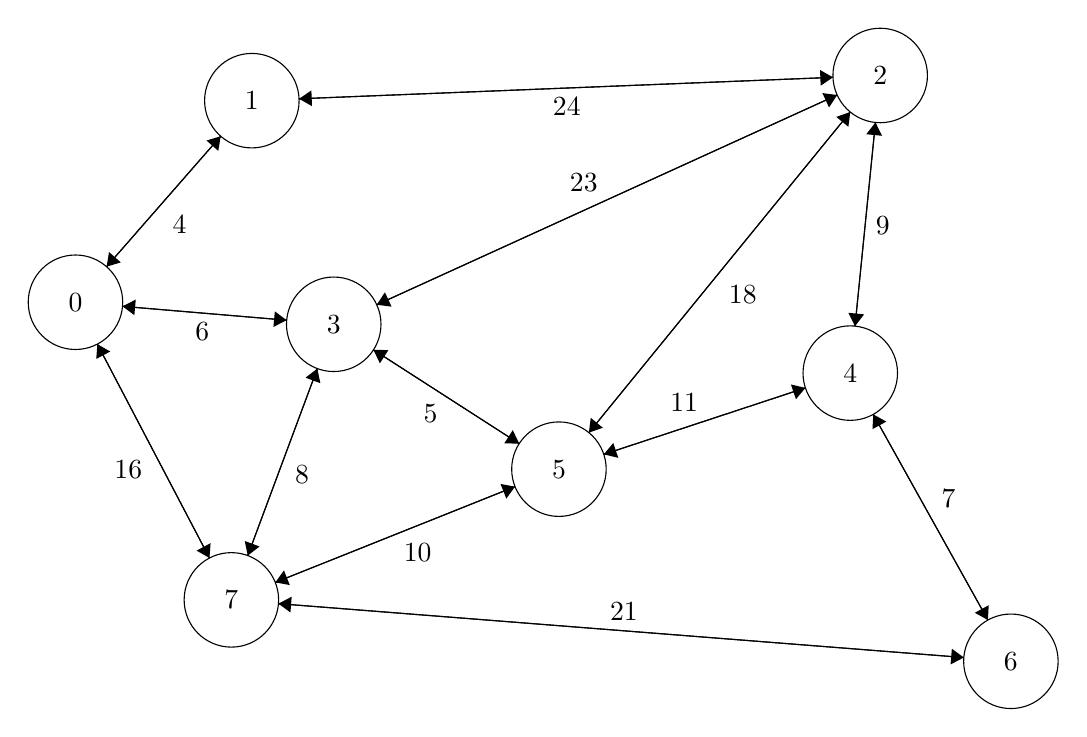
\begin{tikzpicture}[scale=0.2]
        \tikzstyle{every node}+=[inner sep=0pt]
        \draw [black] (13.5,-22.3) circle (3);
        \draw (13.5,-22.3) node {$0$};
        \draw [black] (24.7,-9.5) circle (3);
        \draw (24.7,-9.5) node {$1$};
        \draw [black] (64.6,-7.9) circle (3);
        \draw (64.6,-7.9) node {$2$};
        \draw [black] (29.9,-23.7) circle (3);
        \draw (29.9,-23.7) node {$3$};
        \draw [black] (62.7,-26.8) circle (3);
        \draw (62.7,-26.8) node {$4$};
        \draw [black] (44.2,-32.9) circle (3);
        \draw (44.2,-32.9) node {$5$};
        \draw [black] (72.9,-45.1) circle (3);
        \draw (72.9,-45.1) node {$6$};
        \draw [black] (23.4,-41.2) circle (3);
        \draw (23.4,-41.2) node {$7$};
        \draw [black] (14.89,-24.96) -- (22.01,-38.54);
        \fill [black] (22.01,-38.54) -- (22.08,-37.6) -- (21.19,-38.07);
        \draw (17.77,-32.9) node [left] {$16$};
        \draw [black] (16.49,-22.56) -- (26.91,-23.44);
        \fill [black] (26.91,-23.44) -- (26.16,-22.88) -- (26.07,-23.87);
        \draw (21.56,-23.57) node [below] {$6$};
        \draw [black] (15.48,-20.04) -- (22.72,-11.76);
        \fill [black] (22.72,-11.76) -- (21.82,-12.03) -- (22.57,-12.69);
        \draw (19.64,-17.35) node [right] {$4$};
        \draw [black] (27.7,-9.38) -- (61.6,-8.02);
        \fill [black] (61.6,-8.02) -- (60.78,-7.55) -- (60.82,-8.55);
        \draw (44.7,-9.26) node [below] {$24$};
        \draw [black] (61.6,-8.02) -- (27.7,-9.38);
        \fill [black] (27.7,-9.38) -- (28.52,-9.85) -- (28.48,-8.85);
        \draw [black] (22.72,-11.76) -- (15.48,-20.04);
        \fill [black] (15.48,-20.04) -- (16.38,-19.77) -- (15.63,-19.11);
        \draw [black] (26.91,-23.44) -- (16.49,-22.56);
        \fill [black] (16.49,-22.56) -- (17.24,-23.12) -- (17.33,-22.13);
        \draw [black] (22.01,-38.54) -- (14.89,-24.96);
        \fill [black] (14.89,-24.96) -- (14.82,-25.9) -- (15.71,-25.43);
        \draw [black] (41.68,-31.28) -- (32.42,-25.32);
        \fill [black] (32.42,-25.32) -- (32.83,-26.18) -- (33.37,-25.34);
        \draw [black] (32.42,-25.32) -- (41.68,-31.28);
        \fill [black] (41.68,-31.28) -- (41.27,-30.42) -- (40.73,-31.26);
        \draw (36.05,-28.8) node [below] {$5$};
        \draw [black] (28.86,-26.51) -- (24.44,-38.39);
        \fill [black] (24.44,-38.39) -- (25.19,-37.81) -- (24.25,-37.46);
        \draw [black] (24.44,-38.39) -- (28.86,-26.51);
        \fill [black] (28.86,-26.51) -- (28.11,-27.09) -- (29.05,-27.44);
        \draw (27.41,-33.26) node [right] {$8$};
        \draw [black] (26.19,-40.09) -- (41.41,-34.01);
        \fill [black] (41.41,-34.01) -- (40.49,-33.84) -- (40.86,-34.77);
        \draw (35.23,-37.58) node [below] {$10$};
        \draw [black] (41.41,-34.01) -- (26.19,-40.09);
        \fill [black] (26.19,-40.09) -- (27.11,-40.26) -- (26.74,-39.33);
        \draw [black] (26.39,-41.44) -- (69.91,-44.86);
        \fill [black] (69.91,-44.86) -- (69.15,-44.3) -- (69.07,-45.3);
        \draw [black] (69.91,-44.86) -- (26.39,-41.44);
        \fill [black] (26.39,-41.44) -- (27.15,-42) -- (27.23,-41);
        \draw (48.33,-42.55) node [above] {$21$};
        \draw [black] (47.05,-31.96) -- (59.85,-27.74);
        \fill [black] (59.85,-27.74) -- (58.93,-27.52) -- (59.25,-28.46);
        \draw [black] (59.85,-27.74) -- (47.05,-31.96);
        \fill [black] (47.05,-31.96) -- (47.97,-32.18) -- (47.65,-31.24);
        \draw (52.15,-29.29) node [above] {$11$};
        \draw [black] (64.16,-29.42) -- (71.44,-42.48);
        \fill [black] (71.44,-42.48) -- (71.49,-41.54) -- (70.61,-42.02);
        \draw [black] (71.44,-42.48) -- (64.16,-29.42);
        \fill [black] (64.16,-29.42) -- (64.11,-30.36) -- (64.99,-29.88);
        \draw (68.46,-34.75) node [right] {$7$};
        \draw [black] (32.63,-22.46) -- (61.87,-9.14);
        \fill [black] (61.87,-9.14) -- (60.93,-9.02) -- (61.35,-9.93);
        \draw [black] (61.87,-9.14) -- (32.63,-22.46);
        \fill [black] (32.63,-22.46) -- (33.57,-22.58) -- (33.15,-21.67);
        \draw (45.78,-15.29) node [above] {$23$};
        \draw [black] (46.1,-30.58) -- (62.7,-10.22);
        \fill [black] (62.7,-10.22) -- (61.81,-10.53) -- (62.58,-11.16);
        \draw (54.96,-21.83) node [right] {$18$};
        \draw [black] (62.7,-10.22) -- (46.1,-30.58);
        \fill [black] (46.1,-30.58) -- (46.99,-30.27) -- (46.22,-29.64);
        \draw [black] (63,-23.82) -- (64.3,-10.88);
        \fill [black] (64.3,-10.88) -- (63.72,-11.63) -- (64.72,-11.73);
        \draw (64.29,-17.44) node [right] {$9$};
        \draw [black] (64.3,-10.88) -- (63,-23.82);
        \fill [black] (63,-23.82) -- (63.58,-23.07) -- (62.58,-22.97);
        \end{tikzpicture}
        \end{center}
        
\end{itemize}


\subsection{Connected components}

Trace \textsc{CountAndLabel} (page 204) on the graph of 13 vertices on the preceding page, using DFS.



\subsection{Graph-processing challenges}

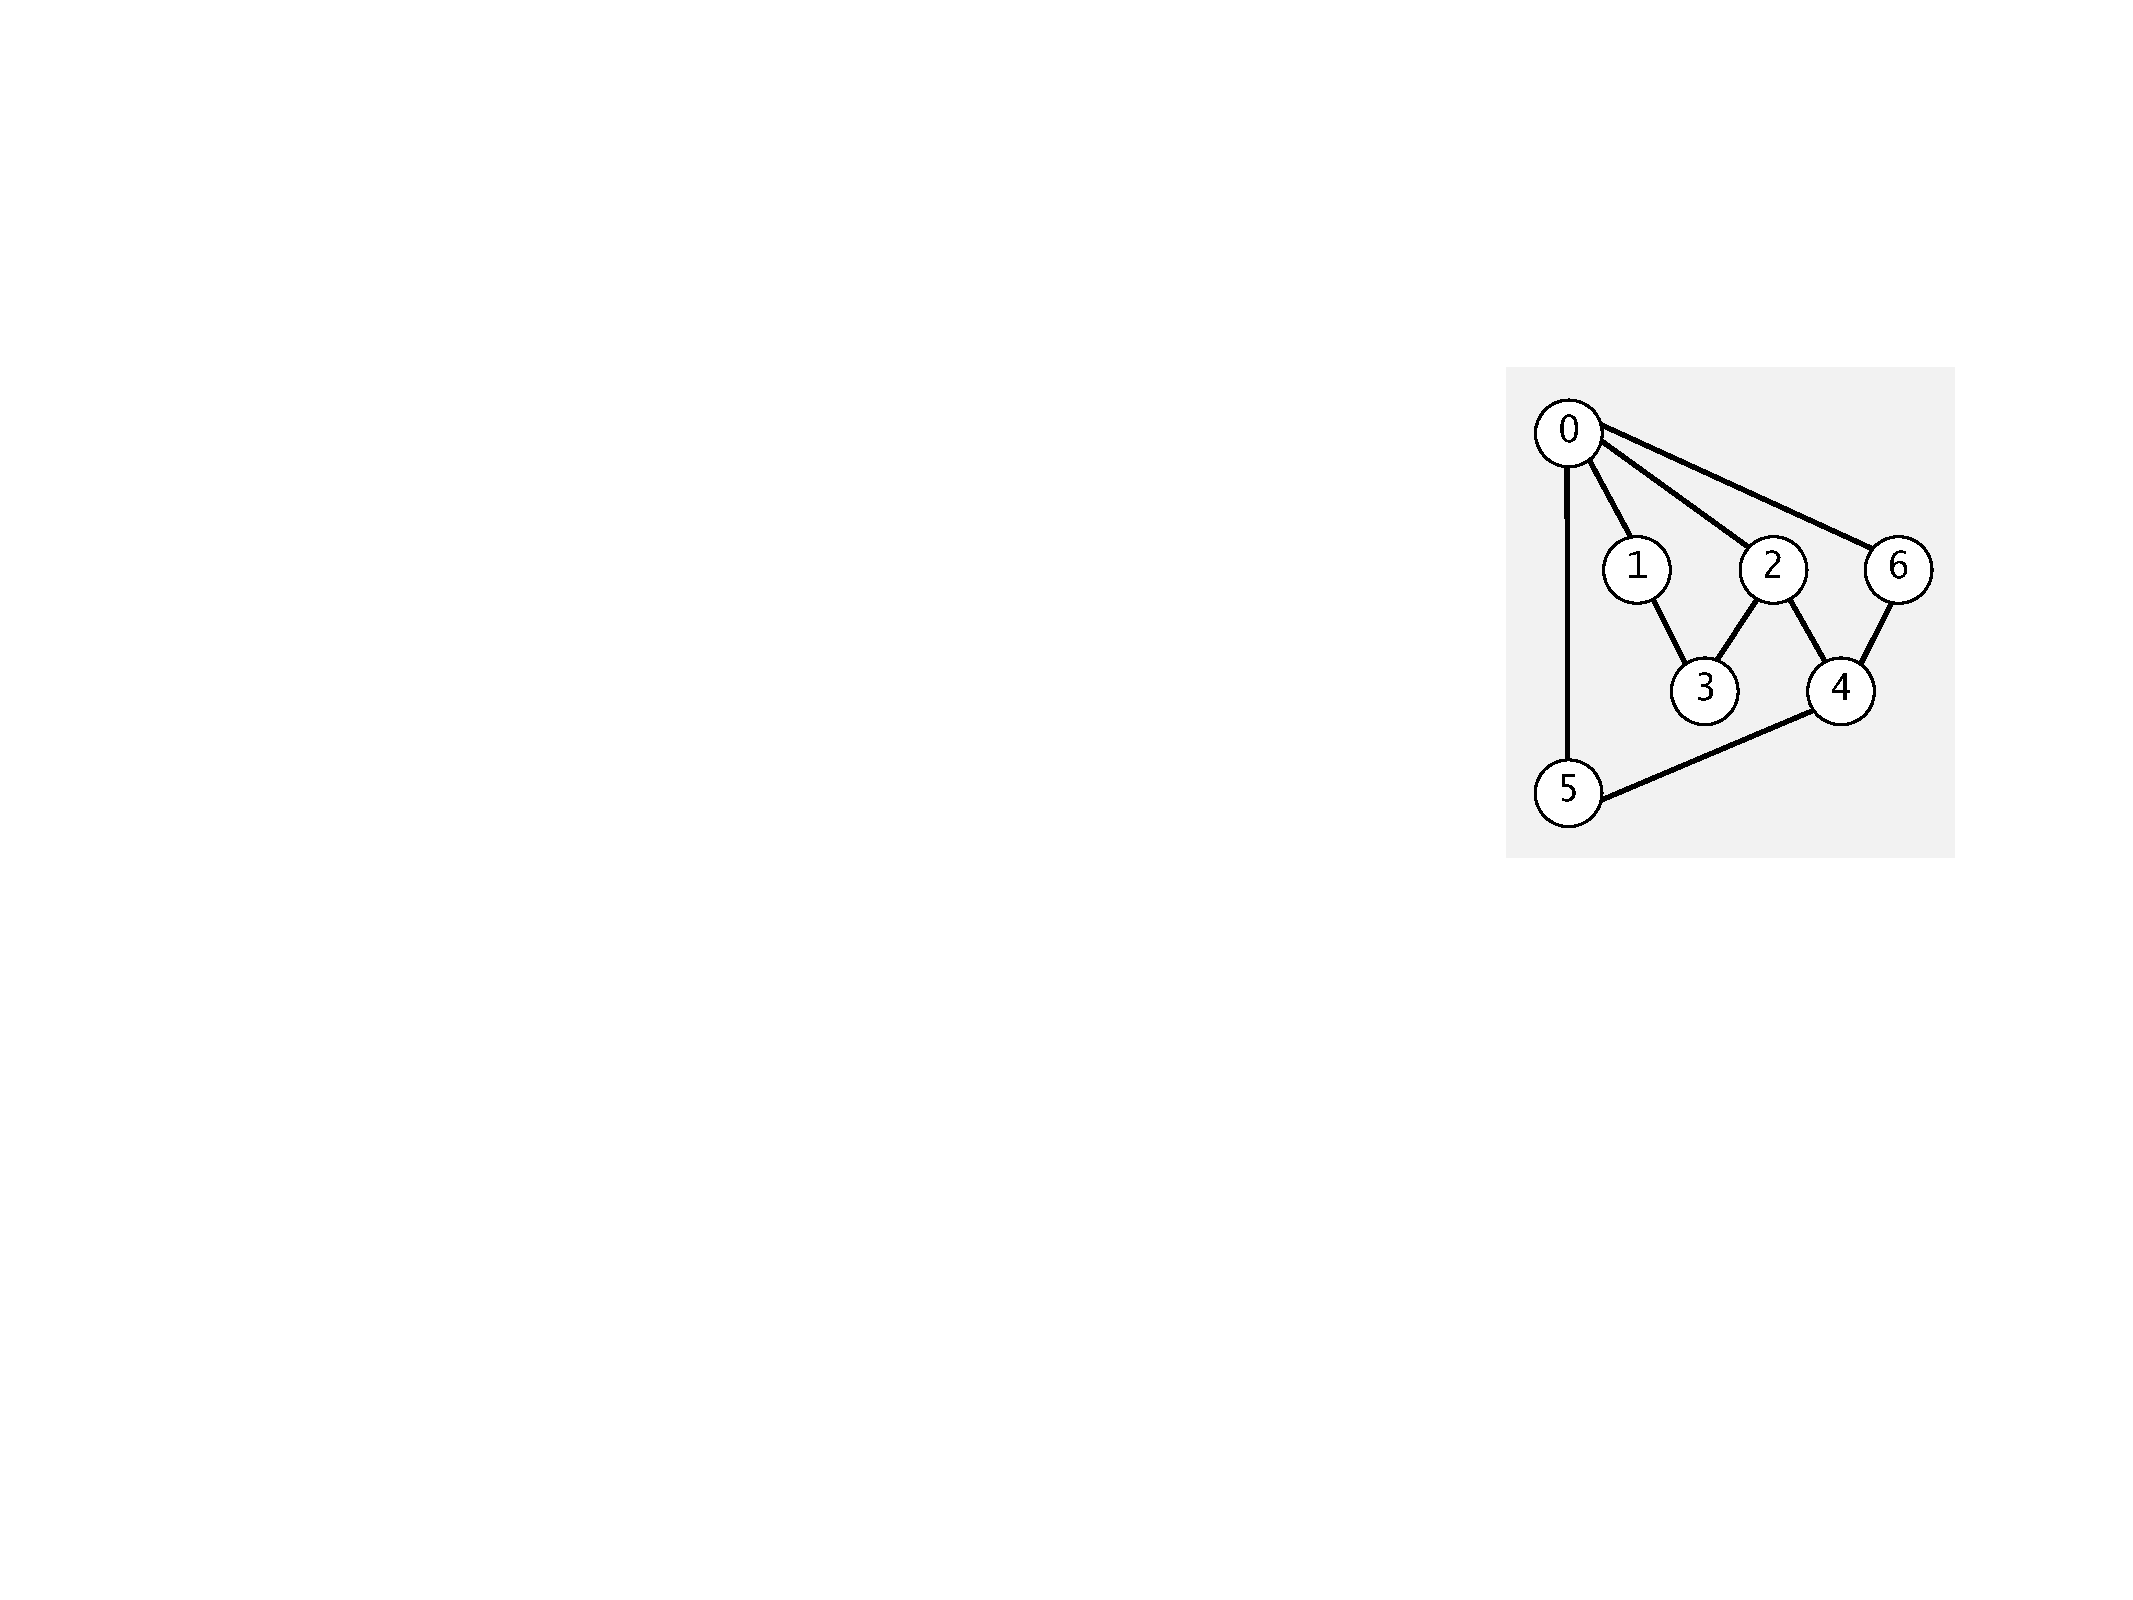
\includegraphics{w07-graph2.pdf}

How difficult?
\begin{itemize}
    \item Any programmer could do it.
    \item Typical diligent algorithms student could do it.
    \item Hire an expert.
    \item Intractable.
    \item No one knows.
    \item Impossible.
\end{itemize}

\subsubsection{Is a graph bipartite?}
\subsubsection{Find a cycle.}
\subsubsection{Find a closed walk that uses every edge exactly once. (Euler cycle)}
\subsubsection{Find a cycle that visits every vertex exactly once. (Hamiltonian cycle)}
\subsubsection{Are two graphs identical except for vertex names? (see next page)}
\subsubsection{Lay out a graph in the plane without crossing edges? (planarity)}

\clearpage
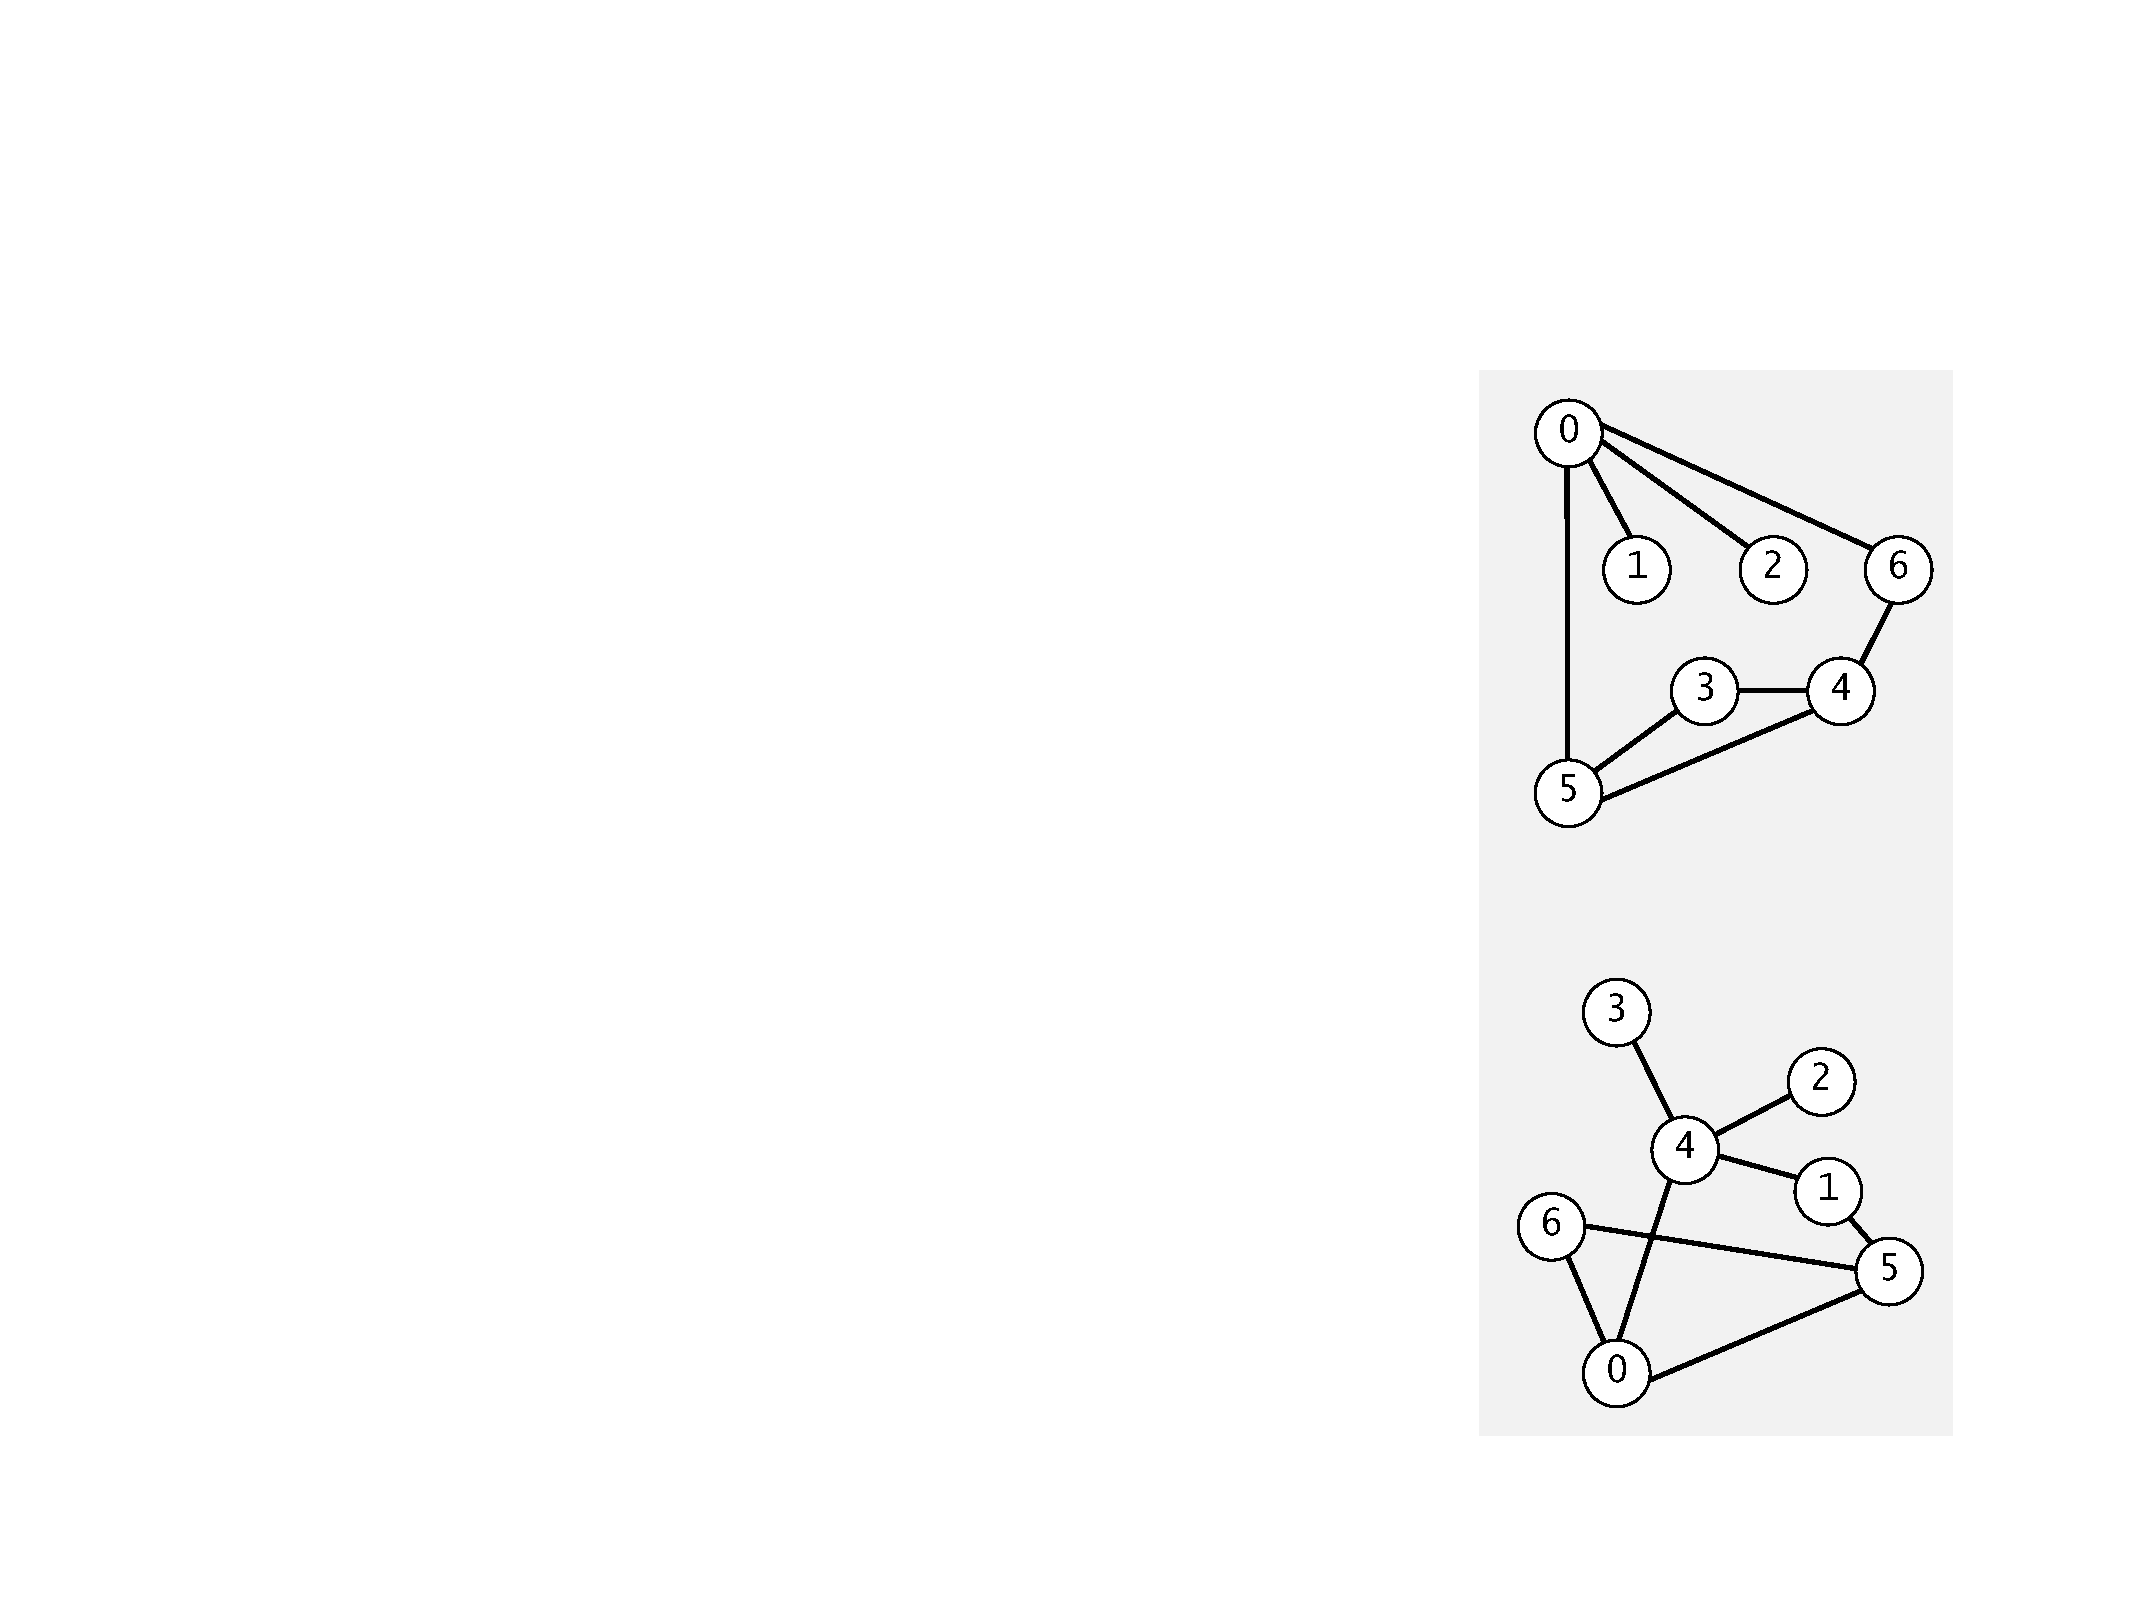
\includegraphics{w07-graph3.pdf}


\clearpage
\subsection{Depth-first search on digraphs}

Trace \textsc{DFSAll} (page 228) on this:
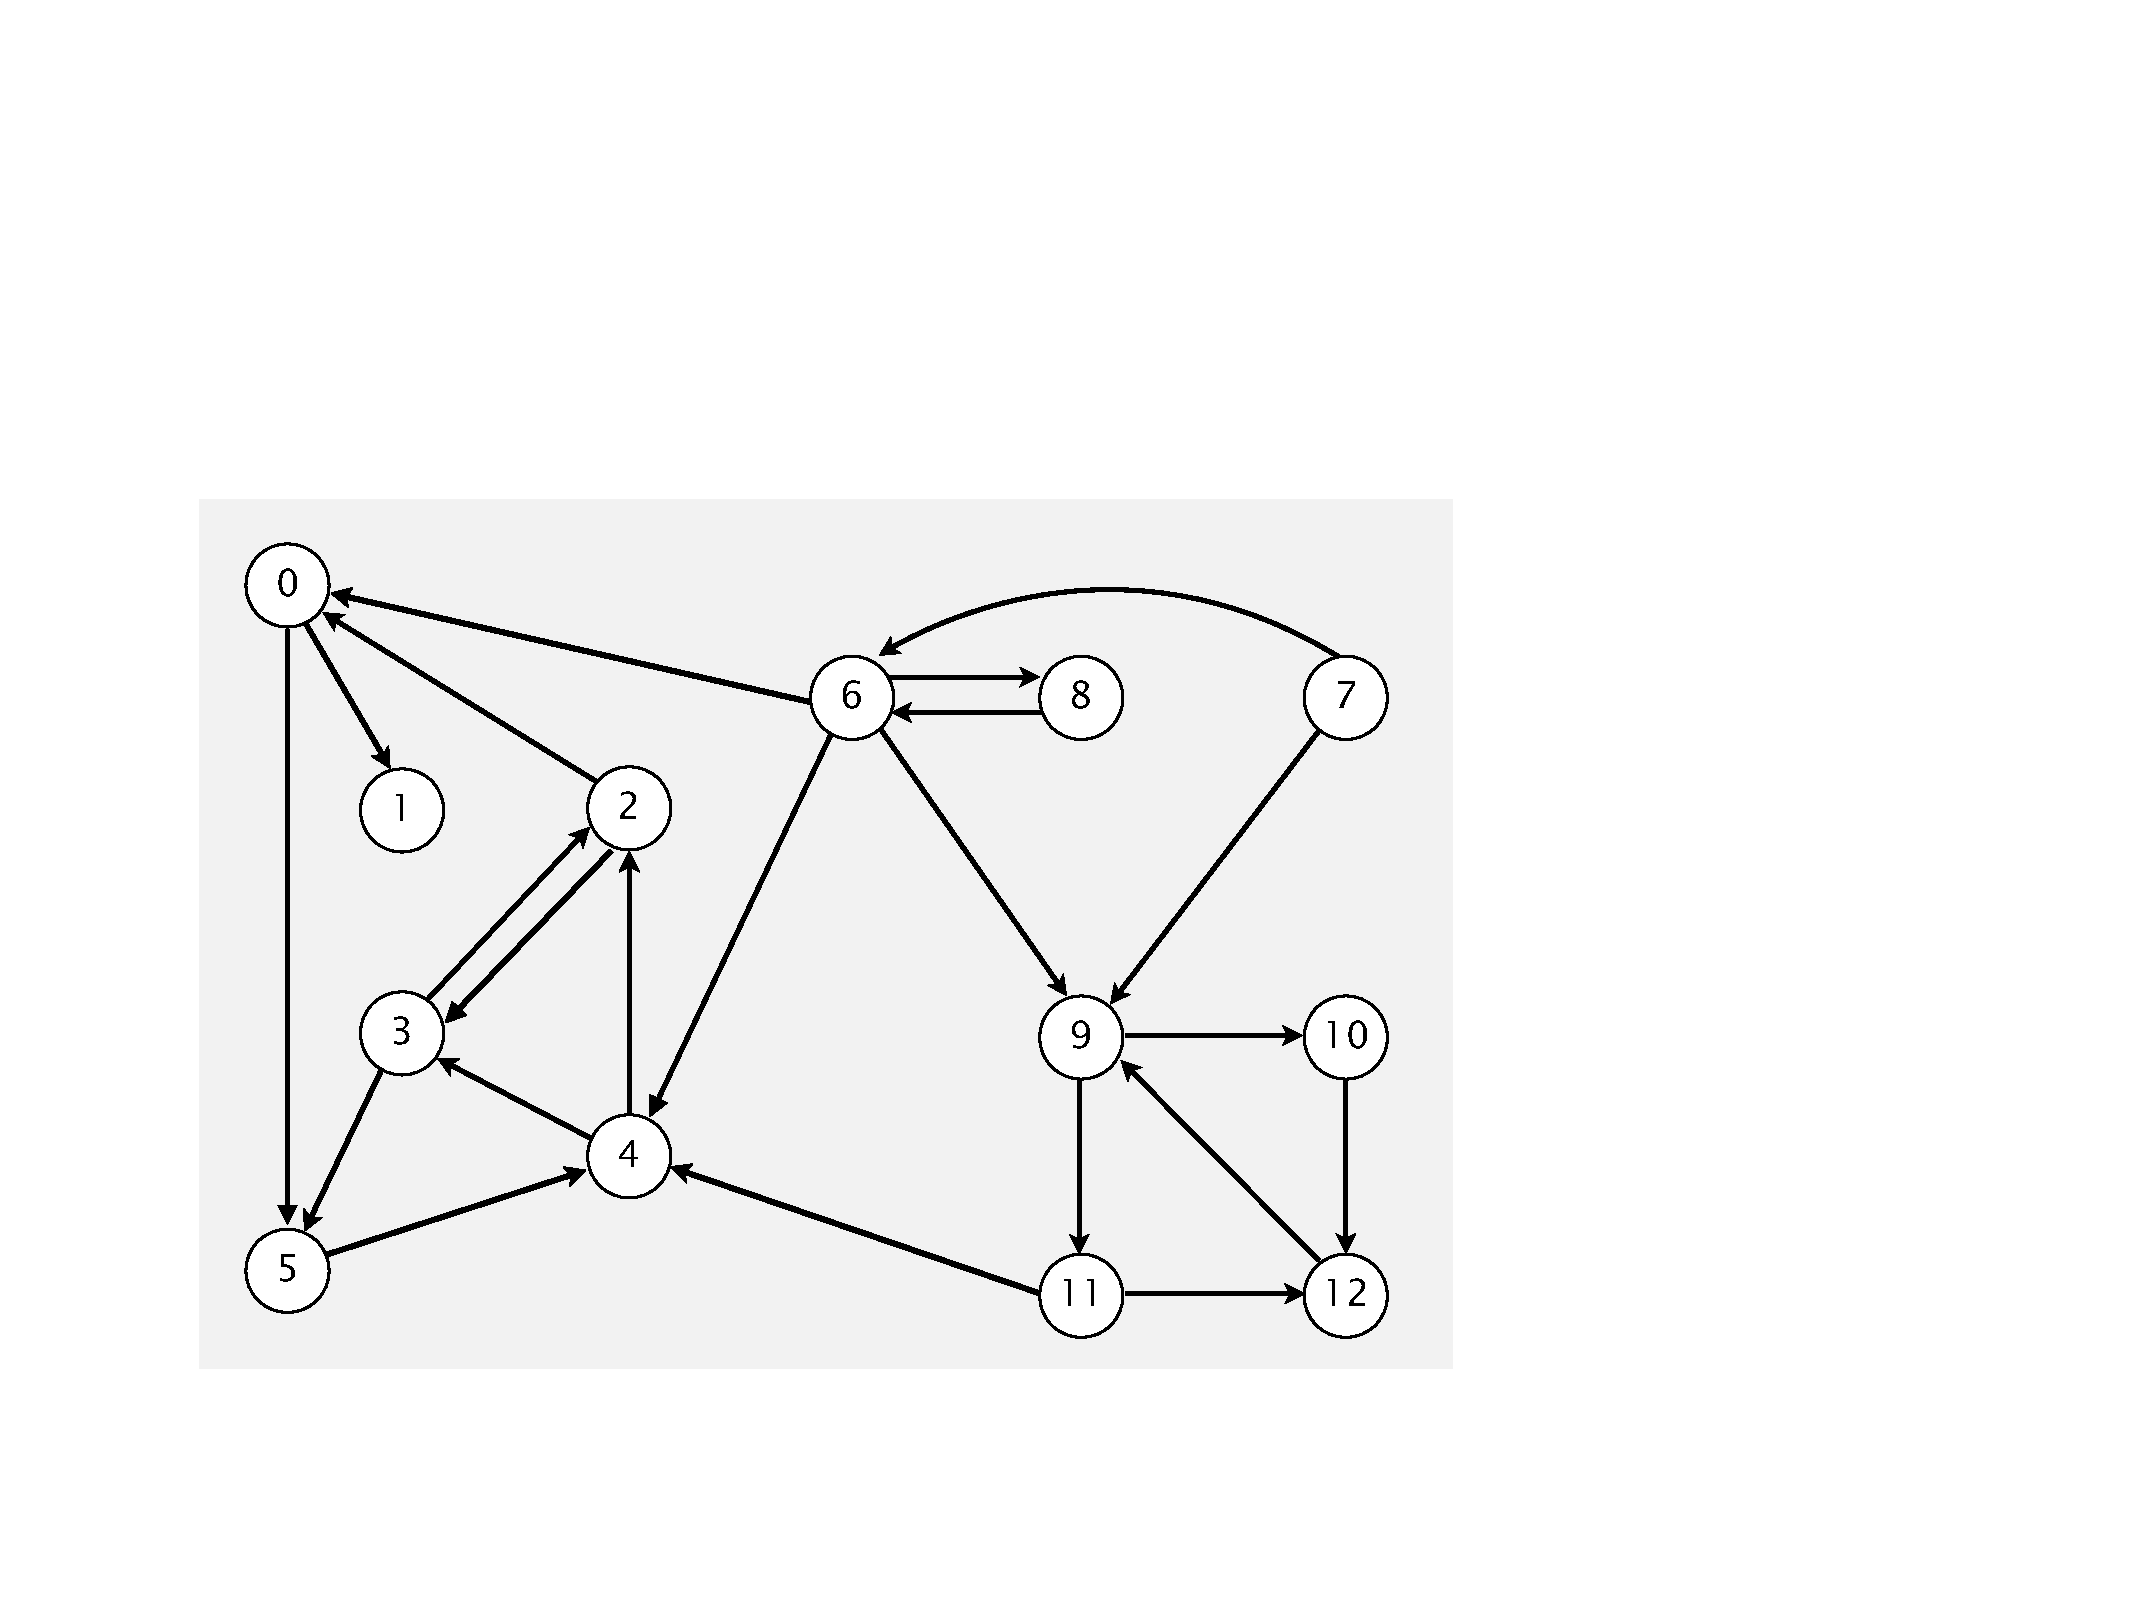
\includegraphics[scale=.5]{w07-graph4.pdf}

Identify different types of edges (tree, forward, back, cross).


\subsection{Topological sort}

\begin{itemize}
    \item Run DFS
    \item Return vertices in reverse postorder
\end{itemize}
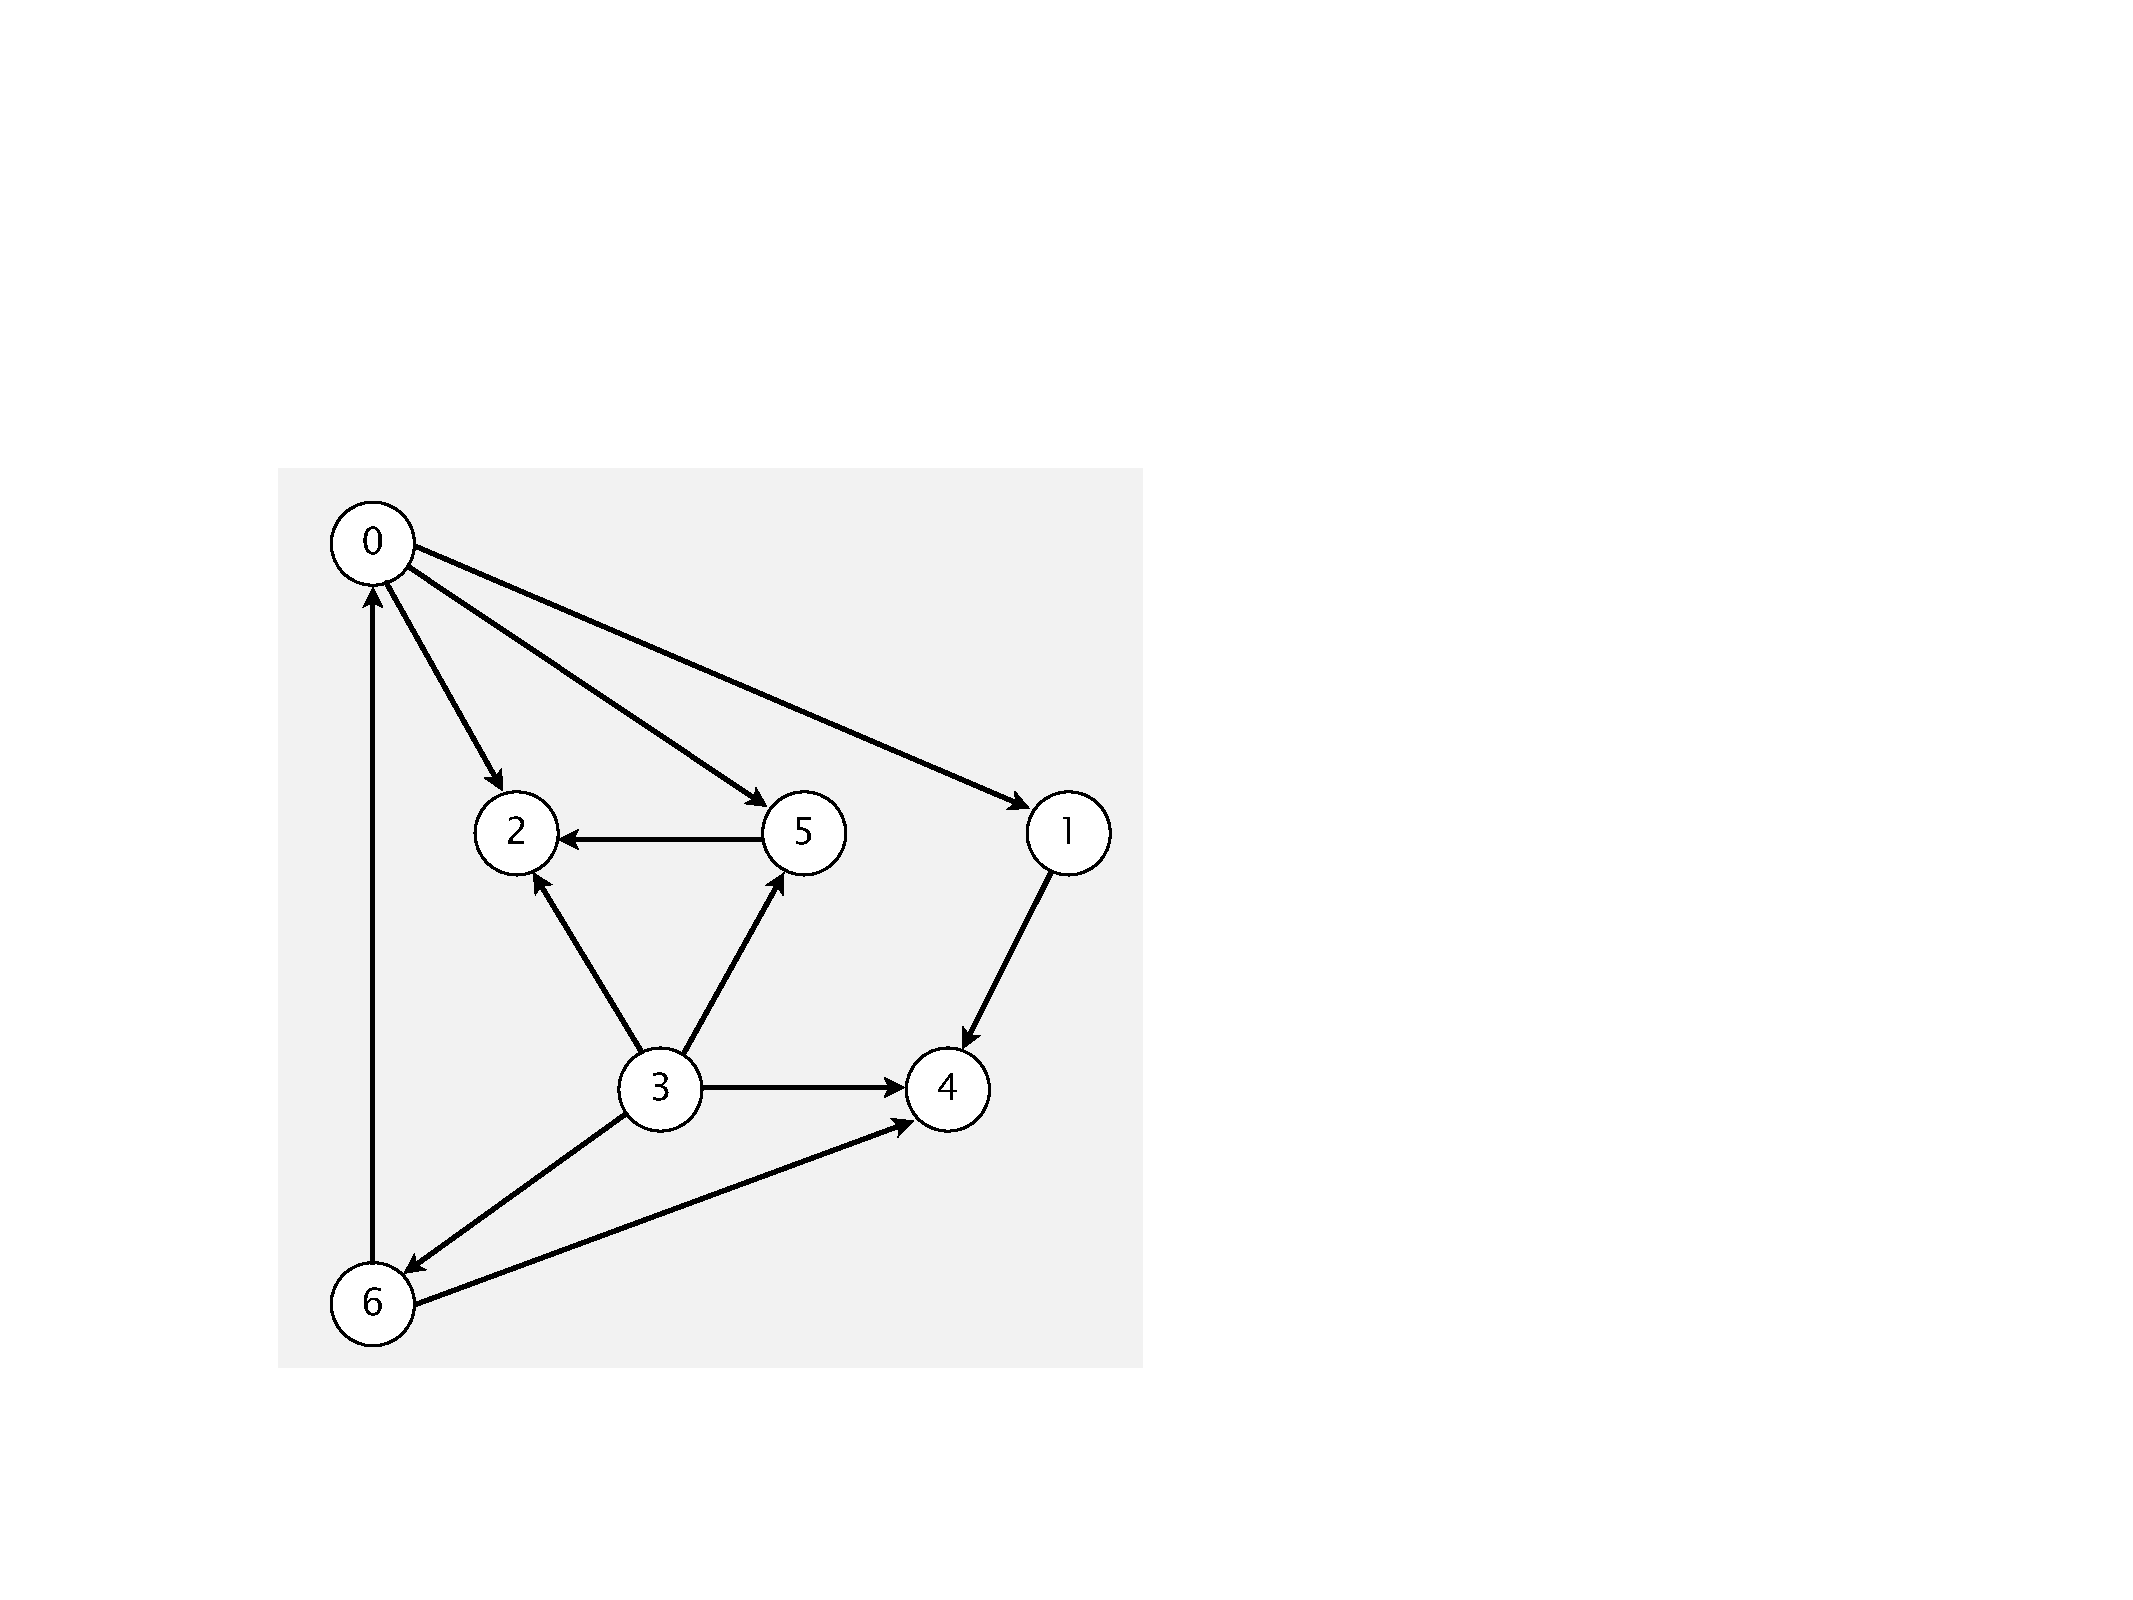
\includegraphics[scale=.5]{w07-graph5.pdf}

\clearpage
\subsection{Strong Components}

\subsubsection*{Kosaraju-Sharir algorithm}

Simple (but mysterious) algorithm for computing strong components.
\begin{itemize}
    \item run DFS on $rev(G)$ to compute reverse postorder.
    \item run DFS on G, considering vertices in order given by first DFS.
\end{itemize}

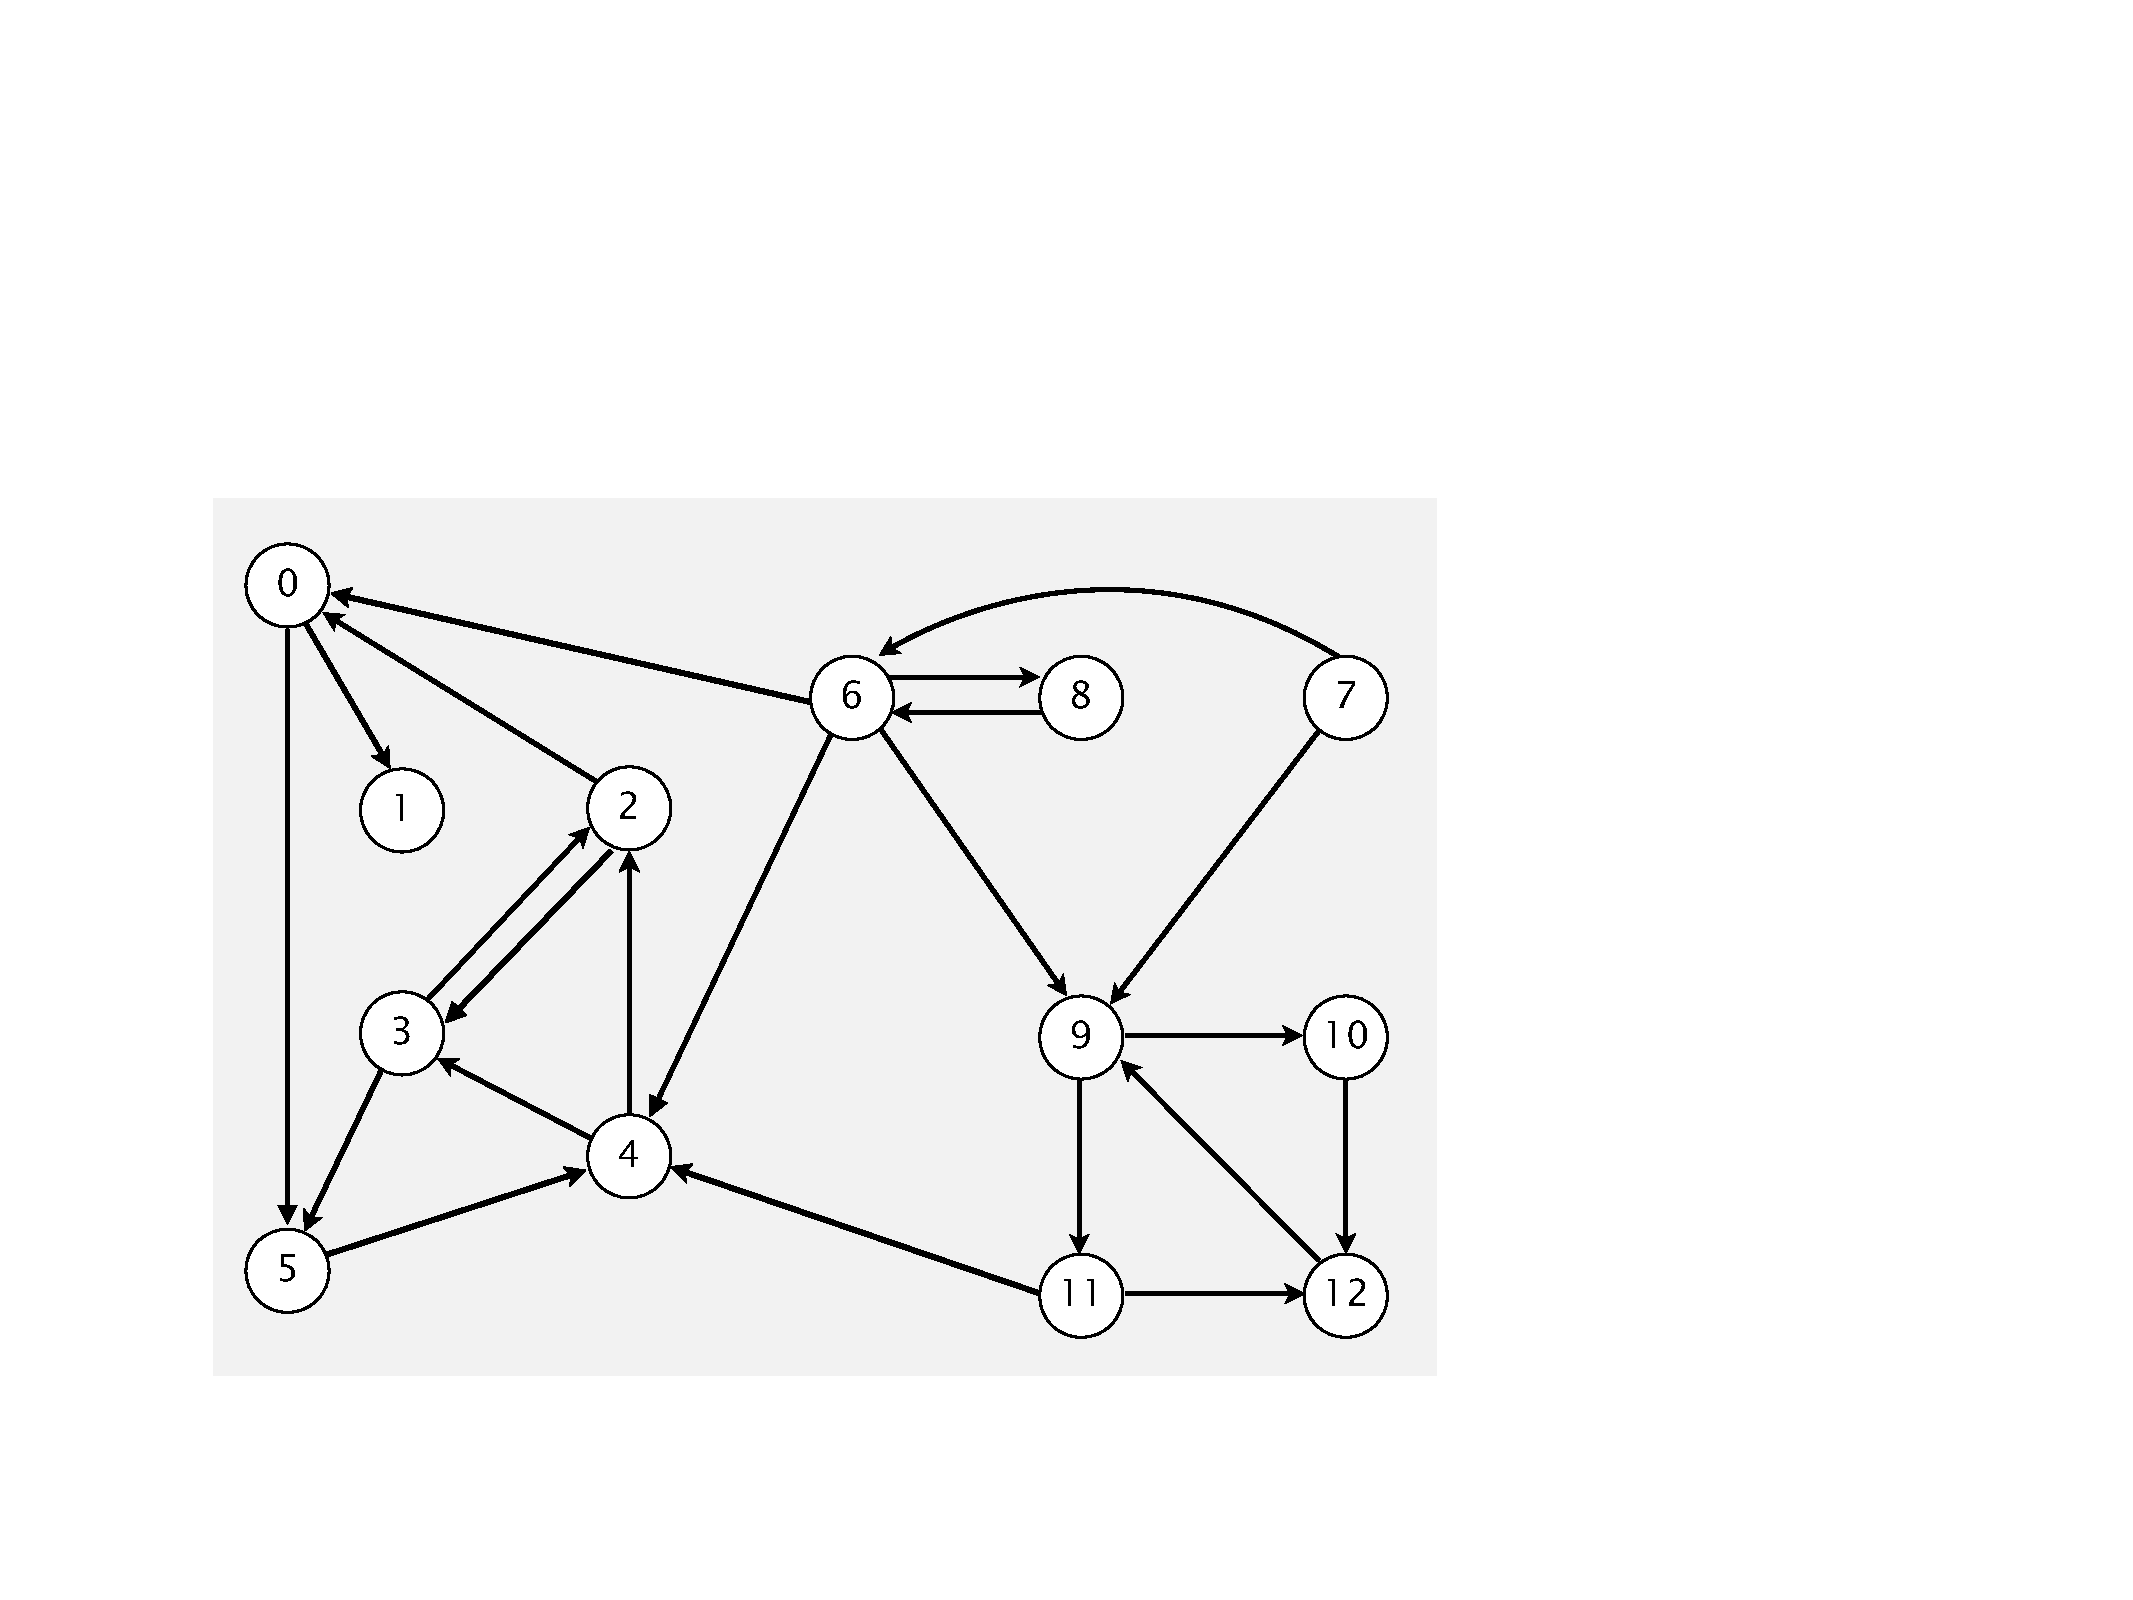
\includegraphics[scale=.5]{w07-graph6.pdf}


\end{document}